
%\keywords{Machine Learning Model Management; Stochastic Gradient Descent; Machine Learning Systems}

\section{Introduction} \label{introduction}
A machine learning pipeline consists of a set of data processing steps, chained together, that result in a machine learning model.
To fully utilize the model,  the model and the pipeline have to be deployed into an environment where they are used to answer prediction queries in real-time.
Continuous training and maintenance of such pipelines are necessary to guarantee an acceptable prediction accuracy.
Many platforms, e.g., Velox \cite{crankshaw2014missing}, Clipper \cite{crankshaw2016clipper}, Laser \cite{agarwal2014laser}, and TensorFlow Serving \cite{abadi2016tensorflow}, have been proposed to provide support for deployment and continuous training of machine learning pipelines. 
However, the platforms mentioned above lack the ability to provide support for continuous and automatic improvement of the pipelines.
Although they provide support for seamless deployment of pipelines, they rely on the users to continuously improve the pipeline and make adjustments.

\begin{figure}[t]
\centering
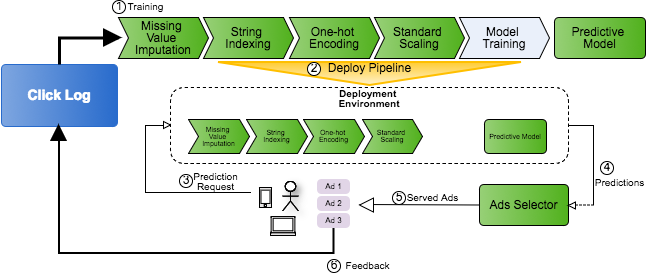
\includegraphics[width=\columnwidth]{../images/motivational-example.png}
\caption{Ads Serving Scenario}
\label{fig:motivational-example}
\end{figure}
\textbf{Example Application.} 
Online advertising is a multi-billion industry.
An advertising network receives ads from different businesses (ads providers) and shows them on different websites (publishers).
Typically, businesses are charged based on the number of clicks users make on their published ads.
Advertising networks use machine learning pipelines to estimate the click rate of different ads.
Figure \ref{fig:motivational-example} shows the work flow of an advertising firm.
The input data (Click Log) consists of several numerical and categorical variables related to the user, publisher's website,  the ads,  and whether or not the users clicked on those ads.
\textcircled{1} A basic click rate prediction pipeline contains the following components:
\begin{itemize}
\item A \textbf{missing value imputer} replaces missing values with appropriate values
\item A \textbf{label indexer} finds the different unique values in a categorical feature 
\item A \textbf{one-hot encoder} creates a new binary feature for every unique value in a categorical feature
\item \hl{A \textbf{data bucketizer} transforms continuous variables into a series of binary variables}
\item A \textbf{standard scaler} scales the data columns to have unit standard deviation and zero mean
\item An finally a \textbf{logistic regression model} is trained using Stochastic Gradient Descent (SGD) optimization technique
\end{itemize}
The pipeline is trained on the click log dataset.
Once the pipeline is created, \textcircled{2} it is deployed into a platform to be used in production.
\textcircled{3} Whenever a user visits a publisher website, a series of prediction queries are sent to the deployment system where the pipeline is used to \textcircled{4} estimate the click rate of the user for the available ads on the website.
\textcircled{5} Ads with the highest click rate estimates are then shown to the user.
Depending on whether the user clicks on the ad or not, \textcircled{6} the platform generates new training data.
The new training data is combined with the existing click log.
The pipeline is periodically (typically on a daily basis) retrained using the data collected by the deployment platform.

The example above demonstrates the complex work flow of a deployment platform.
The deployment platform must be able to guarantee predictions with high accuracy and low latency.
Moreover, it must accommodates all the requests and new training data arriving at the system. 
Our goal is to design a deployment platform that can handle such traffic and provide more accurate predictions to the end user.

\textbf{Existing Deployment methods.} 
To ensure high quality predictions, pipelines should be frequently updated.
Platforms such as Velox update the pipeline in real-time.
However, real-time updates alone are not enough to guarantee a high accuracy for the predictions as they introduce a small amount of error overtime\cite{crankshaw2014missing}.
As a result, the deployed pipelines are periodically retrained offline when the quality of the model goes below a threshold.
Other platforms, such as Clipper and TensorFlow Serving do not offer real-time training.
They operate on the assumption that pipelines are always created and trained offline.
Once the pipelines are trained, they are deployed into these platforms.
Data scientists must continuously enhance the existing pipeline offline and redeploy them into the platform upon a decrease in the quality of the predictions.

In both operation modes (batch only, combined batch/real-time), the overhead of offline training is large and updated pipelines are not immediately available in the deployment environment.
Therefore, predictions made by the platform do not consider the most recent training data.
Moreover, in order not to stall the prediction query answering capabilities of the deployment platforms, offline training is performed outside of the deployment platform.
As a result, the information collected during the online processing is not available for the offline training. 
The offline retraining is a reactive process and it is triggered by a drop in quality or a considerable increase in the amount of available training data.
Based on the amount of the data, the retraining process can take up to hours.
We realized, by replacing the reactive retraining with a series of (proactive) mini-batch trainings, we are able to more rapidly adjust the pipeline.

Proactive training guarantees a higher average quality since the pipeline is updated more frequently.
Moreover, by collecting statistics during the online processing of the data, we can speed up the training.
We propose a hybrid architecture for a deployment platform that supports both real-time and proactive (offline) training of the deployed pipeline.
The architecture enables for two key optimizations.

\textit{Optimization 1.} 
We gather statistics during the online processing of the data. 
These statistics allow us to make the offline training more efficient since calculating them requires a complete scan of the entire dataset.
In our motivating example, label indexing, one-hot encoding, data bucketing, and standard scaling require statistics in form of the mean, standard deviation, and distribution of the features.

\textit{Optimization 2.}
The underlying optimization technique (SGD) for the offline training is an iterative algorithm.
Individual iterations are independent and are typically light weight.
By exploiting these two features of SGD, we replace the time-consuming and resource intensive reactive batch training of the pipeline by a series of single iterations of SGD that are scheduled to execute proactively.

Our experiments show that proactive training of the pipelines achieves more accurate predictions overtime and requires less resources when compared to reactive retraining.

In summary our contributions are:
\begin{itemize}
\item A hybrid architecture for machine learning pipeline deployment platform that caters to both online and offline learning
\item Efficient training of the machine learning pipeline using statistics calculated during the online data processing
\item Removing the overhead of reactive offline training by replacing it with proactive mini-batch training
\end{itemize}

The rest of this paper is organized as follows:
Section \ref {related-work} discusses related work.
In Section \ref{sgd}, we describe the underlying optimization method.
Section \ref{continious-training-serving} and \ref{sec:system-architecutre} introduce the design principles and architecture of our deployment system.
In Section \ref{evaluation}, we evaluate our system against different workloads and compare the performance of our method to other model deployment and maintenance approaches. 
Finally, Section \ref{conclusion} presents our conclusion and future work.
%
%\begin{figure}[t]
%\centering
%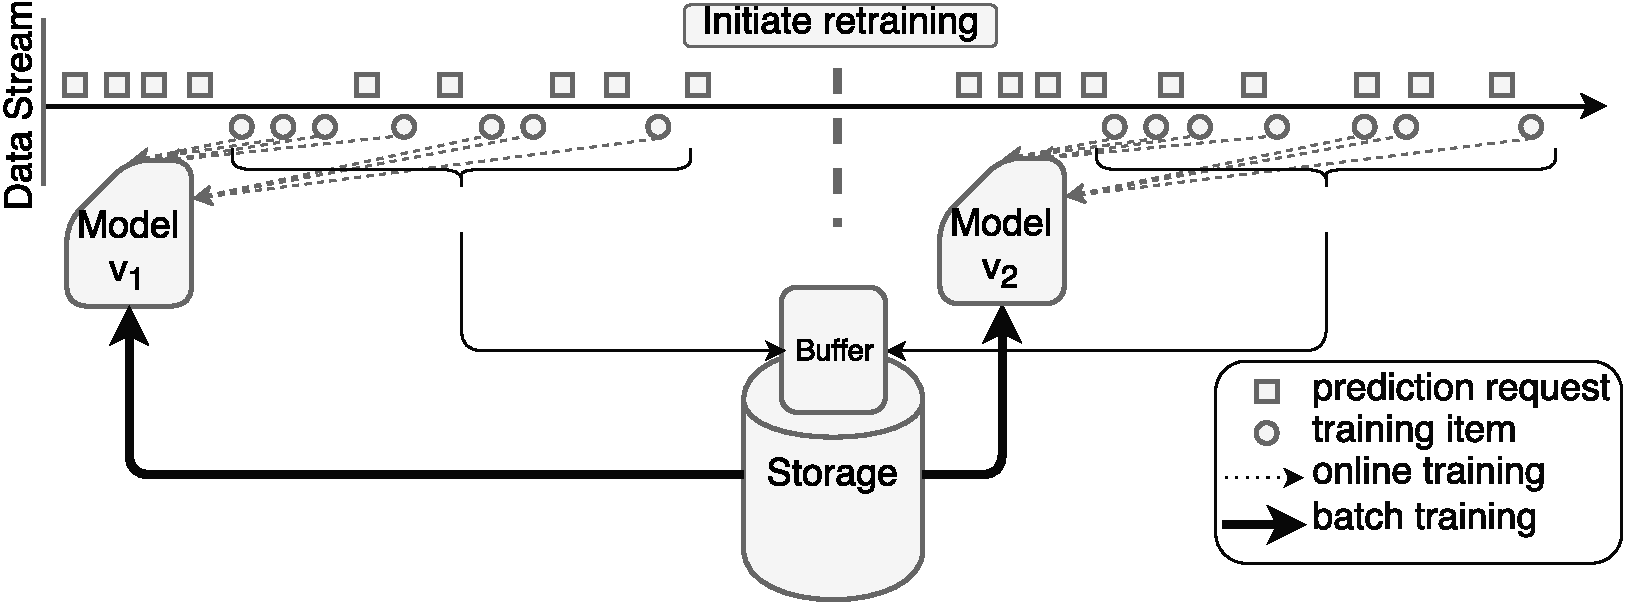
\includegraphics[width=1\columnwidth]{../images/velox-final.pdf}
%\caption{Current Model Deployment Method}
%\label{fig:velox-work-flow}
%\end{figure}


